\section*{Results and Discussion}


%%%%%%%%%%%%%%%%%%%%%%%%%%%%%%%%%%%%%%%%%%%%%%%%%%%%%%%%%%%%
\renewcommand{\arraystretch}{1.1}
\begin{table}[tb]

\begin{center}
 \caption[]{Pairwise $F_{ST}$ among populations \hspace*{2.3cm}}
  \textbf{}\\[-2mm]
{\fontsize{7}{9}\sf
    \begin{tabular}{llccccccl}
    \hline
    & & \\[-3mm]
	&		&	\multicolumn{2}{c}{Mexico}		&	\multicolumn{2}{c}{South America}		\\
	&		&	Lowlands	&	Highlands	&	Lowlands	&	Highlands	\\
      \hline
    & & \\[-3mm]
Mexico	&	Lowlands	&	--	&		&		&		\\
	&	Highlands	&	0.0244	&	--	&		&		\\
SA	&	Lowlands	&	0.0227	&	0.0343	&	--	&		\\
	&	Highlands	&	0.0466	&	0.0534	&	0.0442	&	--	\\ [1mm]
    \hline
	\multicolumn{6}{l}{SNPs from GBS data were used with $2n\geq20$ for each population.}
    \end{tabular}
    \label{FstP}  % caption is needed to make this work
}
\end{center}
\end{table}
\renewcommand{\arraystretch}{1}
%%%%%%%%%%%%%%%%%%%%%%%%%%%%%%%%%%%%%%%%%%%%%%%%%%%%%%%%%%%%

\subsection*{Population structure}

We performed a {\sf STRUCTURE} analysis  \cite[]{Pritchard_2000_10835412,Falush_2003_12930761} 
using MaizeSNP50 data due to its lower error rate for genotyping heterozygotes. 
Accurate estimates of allele frequencies are necessary for this analysis because populations are inferred by minimizing deviations from HWE.
The number of groups was varied from $K=2\sim6$ and the likelihood given $K$ reached a plateau at $K=3$ (Supp FigX).
Several observations can be made based on results from $K=2\sim4$. 
First, most landraces were assigned to groups consistent with our \emph{a priori} population definitions.
Second, while admixture between highland and lowland groups was apparent at intermediate elevations ($\sim1700$m) in both Mexico and South America, greater highland/lowland differentiation was observed in South America.  
Strong divergence of South American highland landraces was supported by their relatively high level of differentiation ($F_{ST}$) from other populations at noncoding and synonymous sites in the GBS data set and may be indicative of a strong bottleneck during colonization of this region.
Third, the Mexican lowland population shared ancestry with both the Mexican highland and South American lowland populations, consistent with a previously described scenario for maize diffusion \cite[]{Piperno_2006_69}.  
Finally, Mexican and South American highland landraces were consistently assigned to separate groups suggesting strong differentiation between maize in these regions.

%\jri{ testing to see if model is robust to amount of gene flow might be easy to do?}
%\comst{check fst with $P_{mex} = 10\%$!!}

%{\sf STRUCTURE} results in Fig.~\ref{map}B suggest the level of divergence between low- and highland populations may be higher in South America than in Mexico.
%We next calculated average $F_{ST}$ values among populations at noncoding and synonymous sites from GBS data ($2n\geq20$ for each population; Table~\ref{FstP}).
%Consistent with the results of {\sf STRUCTURE}, the South American highland population showed a relatively high level of differentiation from the other populations.
%\jri{why silent? i don't see it used much anymore, i think because people have enough data that they can separate out synonymous... thoughts?}
%\st{When using only noncoding SNPs, we obtained almost the same result.
%When using only synonymous SNPs, $F_{ST}$ values became slightly smaller (not shown or supp?). Finally, when using non-synonymous SNPs, Fst decreased even further.}
%The JFD calculated from silent sites of GBS data ($2n\geq30$ for each population) showed a similar trend.  Moreover, as is apparent in Figure ~\ref{JFD}, the variance of change in allele frequency between low- and highland populations is much larger in South America than in Mexico.
%Archaeological evidence suggests that population divergence occurred more recently in South America  \cite[]{Piperno_2006_69,Perry_2006_16511492,Grobman_2012_22307642}.  Combined these factors suggest that the South American highland population may have experienced a stronger bottleneck than the Mexican highland population.
 
 %%%%%%%%%%%%%%%%%%%%%%%%%%%%%%%%%%%%%%%%%%%%%%%%%%%%%%%%%%%%
\renewcommand{\arraystretch}{1.1}
\begin{table}[tb]

\begin{center}
 \caption[]{Inference of demographic parameters\hspace*{0.3cm}}
  \textbf{}\\[-2mm]
{\fontsize{7}{11}\sf
    \begin{tabular}{lcccccccl} \hline
       & & \\[-3mm]
     Mexico  & \multicolumn{2}{c}{Model I}  &\multicolumn{2}{c}{Model II}\\[0.1cm]
    \hline
    & & \\[-3mm]
   & Likelihood & $-$5590.33 & Likelihood &  $-$4641.28 \\
  &$\alpha$    & 0.92  & $\alpha$    & 1.5 \\
  &$\beta$ & 0.38  & $\beta$  & 0.75\\ 
  &$\gamma$   & 1        &  $\gamma$   & 1\\ 
      \hline
    & & \\[-3mm]
    South America  & \multicolumn{2}{c}{Model I}  &\multicolumn{2}{c}{Model III}\\[0.1cm]
        \hline
    & & \\[-3mm]
     & Likelihood &  $-$3858.48 & Likelihood &  $-$8016.88 \\
      &$\alpha$    & 0.55           & $\alpha$       & 1.0 \\
      &$\beta$ & 0.97           & $\beta_1$   & 0.64\\ 
      &$\gamma$   & $\geq$60   &  $\beta_2$  & 0.95\\ 
      &                &                     &  $\gamma$       & $\geq$55\\ [1mm]
    \hline
%    \multicolumn{9}{l}{$^{a}$ The groups were based on phylogenetic analysis in fig.~\ref{tree}\emph{A}}\\
    \end{tabular}
    \label{param}  % caption is needed to make this work
}
\end{center}
\end{table}
\renewcommand{\arraystretch}{1}
%%%%%%%%%%%%%%%%%%%%%%%%%%%%%%%%%%%%%%%%%%%%%%%%%%%%%%%%%%%%
% When P_mex=0.1, alpha=1.1, beta = 0.67



\subsection*{Population differentiation under inferred demography}

Demographic parameters were estimated for lowland and highland populations in both Mexico and South America in order to provide a neutral expectation for population differentiation.  
Models were fit (Fig.~\ref{model}) to the observed JFDs using the maximum likelihood method implemented in {\sf dadi} \cite[]{Gutenkunst_2009_19851460}.  
Estimated parameters are listed in Table~\ref{param} and expected JFDs and residuals are shown in Fig.~\ref{JFD}.  
Overall, the observed and expected JFDs were similar in the two models in both Mexico and South America.
However, residuals indicated an excess of rare variants in the observed JFDs in all cases.  We demonstrate below that this factor should not greatly affect our analysis of population differentiation.

Under both Models I and II In Mexico, we found expansion in the highland population to be unlikely.  
The likelihood value of Model lI ($-$4641.28) was much higher than the likelihood of Model I ($-$5590.33) (Table~\ref{param}), providing evidence that introgression from \emph{mexicana} may have been an important factor during the spread of maize into the Mexican highlands. \mbh{It may be worth running an AIC test on these two models to see if the addition of an introgression parameter significantly improves the likelihood}%However, expected JFDs are visually similar. 
%\jri{i have a bit of trouble understanding this.  if the likelihood is much higher, why would the JFDs be identical?  or does "similar" simply mean in some gross overall sense?}  
%\comst{Jeff - JFDs are not identical, though they look identical. } 
A very strong bottleneck followed by population expansion is supported in maize from the South American highlands based on parameterization of Models I and III.  

\subsubsection{GBS data}We identified significantly differentiated SNPs between low- and highland populations by comparing our empirical $F_{ST}$ values to the neutral expectation given inferred demography.
We simulated $10^7$ SNPs using {\sf ms} software \cite[]{Hudson_2002_11847089} and our inferred demographic parameters and calculated \emph{P}-values for population differentiation in our empirical data using simulated $F_{ST}$ values as a null distribution.  
Two parameter sets were employed for both Mexico (Model I and II) and South America (Model I and III) (Table~\ref{param}).
Model choice had little effect in both Mexico and South America (\emph{i.e.,} we obtained very similar null distributions of $F_{ST}$ values (Figure~\ref{FstDist}A)).
Moreover, null and observed distributions of $F_{ST}$ values were quite similar under our tested models (Figure~\ref{FstDist}A).
Thus, although we observed an excess of rare variants in the observed JFDs (Figure~\ref{JFD}), our results should be conservative.

We also tested the robustness of our analysis of population differentiation to the specification of the model.  
%The distributions of calculated \emph{P}-values were also similar between the models both in Mexico and South America (Supp Figure~4).
In addition to the parameters listed in Fig.~\ref{model}, we treated the size of the domestication bottleneck  ($N_B$) as a variable parameter.  
Surprisingly, $N_B$ was estimated to be equal to the population size at the end of the bottleneck, $N_C$ (\emph{i.e.,} no bottleneck was most likely; supp Table~3).  
Moreover, the likelihood was much smaller for a bottleneck model (supp table~3) than for alternative models described in Table~\ref{param}, suggesting a domestication bottleneck did not occur.
This result may at first seem surprising given previous work regarding the demography of maize during domestication.  For example, \cite{Wright_2005_15919994} inferred the strength of the domestication bottleneck by analyzing coding regions and found these to have an excess of SNPs with intermediate allele frequencies, a population signature consistent with a recent bottleneck.  
In contrast, \cite{Hufford_2012_22660546} demonstrated that intergenic regions in maize, unlike coding regions, showed an excess of rare variants.
Our JFDs using SNPs from across the genome (\emph{i.e.}, both genic and intergenic) also showed an excess of rare variants from the expectation under \cite{Wright_2005_15919994}'s bottleneck model.
%Higher density data may be necessary to adequately infer the domestication bottleneck.
The effects of the maize domestication bottleneck may therefore be most apparent in coding regions.
 Nevertheless, presence versus absence of a bottleneck had little effect on distributions of \emph{P}-values for differentiation between highland and lowland maize as shown in supp figure~5.  %, though \emph{P}-values became a bit bigger without the bottleneck. 
%\mbh{what is meant by bigger p-value? More significant (i.e., smaller value)?  Is this really negligible?  Not sure it's necessary to tag this on to the end.}  
 
%\st{Need to explain why?  Stephen used coding regions, but we use SNPs from whole genome.    Oh, this is beyond the scope of our paper!!} \jri{no this is a cool result that needs to stay in the discussion}


\subsubsection{MaizeSNP50 data}To overcome ascertainment bias in the MaizeSNP50 data set, we employed a simple method in which we added two individuals to the Mexican lowland population representing the maize lines B73 and Mo17. For Model I in South America we added two individuals at time $t_F$ to the ancestral population of the South American low- and highland populations because the Mexican lowland population was not incorporated into this model.  Without this modification of our demographic model, we underestimated \emph{P}-values, but the effect was very small (Supp Figure~6).   Furthermore, the empirical and null distributions of $F_{ST}$ values were very similar in the MaizeSNP50 data set despite the fact that multiple ascertainment schemes were used (Figure~\ref{FstDist}B; Supp Figure~6). 

%%%%%%%%%%%%%%%%%%%%%%%%%%%%%%%%%%%%%%%%%% FIGURE
\begin{figure}[tb]   
  \begin{center}
   \vspace{-0mm}
   %\includegraphics[width=0.23\textwidth]{figs/model}
   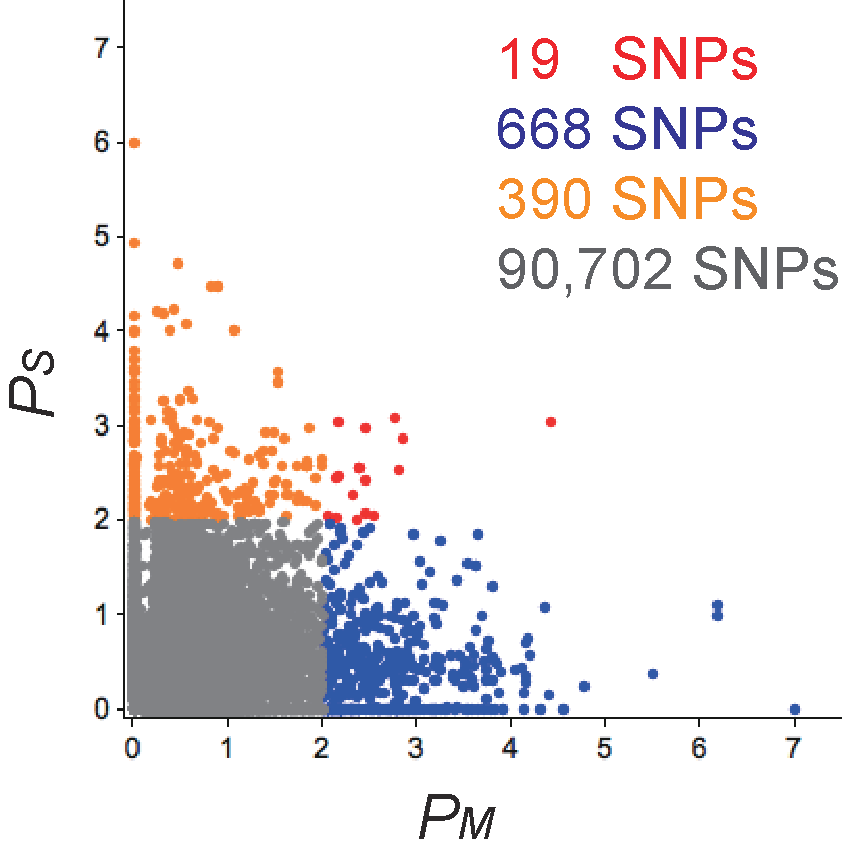
\includegraphics[width=0.4\textwidth]{fig/Fig6}
   \renewcommand{\baselinestretch}{0.9}
   \vspace{-3mm}
   \caption{Scatter plot for \emph{P}-values of population differentiation between low- and highland populations in Mexico ($P_X$ on \emph{x}-axes) and South America ($P_S$ on \emph{y}-axes).  $P_M$ and $P_S$ are scaled by --log$_{10}$.  Red, blue, orange and gray dots represents SNPs showing significance in both Mexico and South America, only in Mexico, only in South America, respectively.} \jri{do we know what that clear outlier red SNP is? anything interesting?}
\vspace{-6mm}
    \label{PvDist}
  \end{center}
\end{figure}
%%%%%%%%%%%%%%%%%%%%%%%%%%%%%%%%%%%%%%%%%% FIGURE




\subsubsection{Joint data set}In total, 91,779 SNPs remained in our joint, filtered GBS and MaizeSNP50 data set ($2n\geq20$ and HWE $P\geq0.005$ \mbh{need to keep track of how this is reported: sometimes 0.005, sometimes 0.5\%} for GBS or $P\geq0.05$ for MaizeSNP50 for all four populations).  For the Mexican and South American populations, we calculated \emph{P}-values for 76,989 and 63,160 SNPs respectively with the remaining SNPs being monomorphic. The reduced number of polymorphic SNPs in South America relative to Mexico is likely due to a lower effective population size in the South American populations.  48,370 SNPs were polymorphic in both Mexico and South America. 


We chose $P<0.01$ as an arbitrary cut-off for significant differentiation between low- and highland populations.  
We found 1,040 SNPs with $P<0.01$ in Mexico (1,040/76,989=0.0135) and 756 in South America (756/63,160=0.0120).  
Expected and observed numbers of significance were almost equal.  
In total, 1,740 SNPs showed significant differentiation in Mexico and/or South America.

\subsection*{Patterns of adaptation}

\subsubsection{Adaptation via mutation versus standing variation}

In order to characterize patterns of adaptation we first determined whether putatively adaptive variants (\emph{i.e.}, highly differentiated SNPs between the lowlands and the highlands) arose primarily through new mutations or standing genetic variation.  
We found that putatively adaptive variants in both Mexico and South America tended to segregate in lowland populations more commonly than the remainder of SNPs (84.6\% vs. 74.8\% in Mexico, FET {$P < 10^{-11}$ and 87.3\% vs 81.8\% in South America,  $P< 10^{-3}$).  
\plr{What does ``adaptive variants tended to segregate'' mean?  That high $F_{ST}$ SNPs are more likely to be polymorphic in those pops?}
We extended this analysis to standing variation in \emph{parviglumis}, the progenitor of domesticated maize, by retrieving genome-wide SNP data from 14 \emph{parviglumis} inbred lines included in the Hapmap v2 data set, using only SNPs with $n\geq10$ \cite[]{Hufford_2012_22660546}.  Again we found that putatively adaptive variants tended to segregate to a disproportionate extent in \emph{parviglumis} (81.1\% vs. 72.1\% in Mexico, FET {$P < 10^{-6}$ and 81.2\% vs 72.7\% in South America,  $P< 10^{-4}$).  \mbh{Sho, I extensively edited the previous sentences of this paragraph.  I was careful to keep all \%'s and $P$-values straight, but might be a good idea to double check} 

\textcolor{red}{It has been demonstrated that the domestication traits in maize were mainly established such that the frequency of maize-type alleles was increased that are maintained at low frequency in teosinte.  \emph{tb1} (who reported this first?) and \emph{gt1} \cite[]{Wills2013} are, for example, the case (and more?).  Our results may extend this view: selection from standing variation are mainly involved in the processes of domestication and local adaptation in maize.  
Recently, the lines of evidence for selection from standing variation is increased in model organisms such as Drosophila (Petrov arXiv) and human \cite[]{Turchin_2012_22902787,Peter_2012_23071458}.}

%compare to above
%\textcolor{red}{It has been demonstrated that the domestication traits in maize were mainly established such that the frequency of maize-type alleles was increased that are maintained at low frequency in teosinte.
%\emph{tb1} \cite[]{Studer_2011_21946354}, \emph{ba1} \cite[]{Gallavotti_2004_15577912}, \emph{ra1} \cite[]{Sigmon_2010_20196812} and \emph{gt1} \cite[]{Wills2013} are, for example, the case.  Our results may extend this view: selection from standing variation are mainly involved in the processes of domestication and local adaptation in maize.


In summary, the progenitor populations of highland maize (lowland maize and \emph{parviglumis}) contain both genotypes of highly differentiated SNPs implying adaptation from standing variation.
However, standing variation may be difficult to distinguish from gene flow between lowland and highland populations due to their recent divergence in units of $N_A$.
An additional caveat is that our inference of adaptation from standing variation assumes that our highly differentiated SNPs are causal and not merely linked to the targets of adaptation.  A causal variant at some distance from the assayed SNP may have had the opportunity to recombine onto multiple backgrounds. 
%I think we can drop this explanation? The more likely one is that we missed stuff entirely, no?
Given the previously documented rapid decay of linkage disequilibrium in maize \cite[]{Tenaillon_2001_11470895,Remington_2001_11562485} that is also apparent in our data (supp fig.~X) we are also likely missing a number of selected loci not in LD with the SNPs assayed here.

\mbh{Please note that I've commented out a large amount of text and comments at this point in the manuscript.  Probably a good idea to read through this to make sure there are not parts that you would like to bring back.}

%\st{(Or we can say without gene flow, we can well explain the observed pattern of polymorphisms).
%Lots of shared polymorphisms between maize and teosinte may support the standing variation hypo? Standing variation hypo holds as long as the effect of gene flow between maize and teosinte is negligible. 
%In fact, \cite{vanHeerwaarden_2011_21189301} estimated admixture between Mexico lowlands maize and \emph{parviglumis} to be very low. 
%Admixture from  \emph{parviglumis} to maize may alter the shape of the null distributions of $F_{ST}$ values.
%We checked even high admixture (up to 20\%) did not change the distributions (\cite{vanHeerwaarden_2011_21189301} estimated a few percentage of admixture).
%Thus, our $F_{ST}$ outlier approach is conservative on gene flow.}

\subsubsection{Highland versus lowland adaptation}

Given the history of the spread of maize, it is tempting to assume that significant population differentiation is due to an increase in frequency of adaptive alleles in the highlands.
However, we cannot rule out the possibility of adaptation in the lowlands.
Therefore we further investigated patterns of allele frequency change across populations.
When data were available for \emph{parviglumis} from Hapmap v2 \cite[]{Chia_2012_22660545,Hufford_2012_22660546}, we included these in our analysis.

First, we assessed patterns of allele frequencies in SNPs that were significantly differentiated between highland and lowland maize.
We focused on SNPs segregating as shown in Fig.~\ref{tes2}A, although some SNPs showed more complex patterns.
The first and second rows show hypothesized patterns of segregation under highland adaptation; here, allele frequencies in maize from a highland region are highly differentiated from those of \emph{parviglumis} and maize from the corresponding lowland region. %and no difference is observed between South America populations.
%When \emph{parviglumis} data are lacking, SNPs showing the pattern of segregation in the third row likely underly highland adaptation.
%\mbh{don't think this row in the figure is necessary}
Similarly, patterns of SNP segregation depicted in the fourth to sixth rows are consistent with lowland adaptation.
%The patterns expected for highland and lowland adaptation in South America are qualitatively the same as those shown for Mexico in Fig.~\ref{tes2}A.
We found that 74.5\% (400/537) and 84.5\%(448/530) of putatively adaptive SNPs in Mexico and South America respectively that displayed segregation patterns consistent with highland adaptation also had lower P-values for the PHS test in highland maize.
Likewise, 63.5\% and 67.1\% of the putatively adaptive SNPs in Mexico and South America that showed segregation patterns consistent with lowland adaptation also showed lower P-values for the PHS test in lowland maize.
Additionally, when a putatively derived allele segregated in both the lowlands and highlands but was more prevalent in the highlands, 67.5\% and 67.6\% of such SNPs showed lower PHS \emph{P}-values in the highlands in Mexico and South America. 
\jri{is this more that show the PHS stat than expected? that is if you pick random alleles, or maybe random alleles at similar frequencies?}
\comst{I tested: $P<10^{-11}, < 0.01$, $\approx 0$, $<10^{-9}$ for Mex high, Mex low, SA high and SA low, respectively}


\subsubsection{Adaptation through introgression}

 A marked difference between highland adaptation of maize in Mexico and South America is the potential for adaptation through introgression from wild relatives.  While maize in Mexico grows in sympatry with both the lowland taxon \emph{parviglumis} and the highland taxon \emph{mexicana}, maize in South America is outside the range of the wild \emph{Zea} species.
 \cite{Pyhajarvi2013} recently assessed the potential for local adaptation in \emph{parviglumis} and \emph{mexicana} populations, characterizing differentiation between these subspecies using an Fst-outlier approach.
%\emph{parviglumis} and \emph{mexicana} inhabit the Mexico lowlands and highlands, respectively, so we expected that some some SNPs highly differentiated between these subspecies would overlap highly differentiated SNPs lowland and highland Mexican maize.
We observed a significant excess of overlap between our putatively adaptive SNPs in Mexican maize and those identified in the \cite{Pyhajarvi2013} analysis (Table~\ref{tanja}; $P<0.01$ by FET).
Significant overlap was also observed with South American maize populations ($P<0.01$), but the proportion of SNPs was lower than observed in Mexico.  These data suggest that adaptations in Mexican maize may have been obtained through gene flow with wild relatives.  To more fully explore this hypothesis we evaluated our data in light of introgression identified by \cite{Profford_2013} from \emph{mexicana} into maize in the Mexico highlands.  
The proportion of significant SNPs in introgressed regions in Mexico is significantly higher than found in South America (Fisher's exact test, $P\ll0.001$).
%When focusing on GUs, we identified 99/586 (14.5\%) and 22/466 (4.7\%) GUs of Mexico- and SA-specific significance in introgressed regions (Fisher's exact test, $P<10^{-6}$). 
\plr{This part is very nice.  I did wonder how different the proportions are?}
Outside introgressed regions, the Mexican and South American populations did not show marked differences in the proportion of significant SNPs (Fisher's exact test, $P>0.7$). %\jri{cool!}  
These trends indicate \emph{mexicana} has played a more substantial role in conferring highland adaptation to maize in Mexico than in South America as would be expected considering the range of \emph{mexicana} does not extend to South America.

\textcolor{red}{One more thing.  The SNPs with significant $F_{ST}$ $P$-values are enriched in intergenic regions than ones with non-significant $P$-values (51.3\% vs. 44.2\%; FET $P < 10^{-8}$).  That would be consistent with the idea that selection on regulatory regions is a predominant force in the maize domestication process (Doebley?). On the other hand, the comparison between nonsynonymous and synonymous SNPs did not show significant difference.  These results are consistent with the results of \cite{Pyhajarvi2013}.}

\subsubsection{Evidence for parallel adaptation}

While maize adaptation in Mexico and South America are likely distinguished by unique histories of gene flow with wild relatives, the potential remains for parallel adaptation in these two regions.  If a SNP showed significant differentiation between low- and highland populations in both Mexico and South America, it was potentially a target of parallel adaptation.  
Let $P_M$ and $P_S$ be \emph{P}-values in Mexico and South America, respectively.
We found 56 SNPs with $P_M<0.01 \cap  P_S<0.01$.  
This number  was significantly larger than the random expectation ($48,370\times 0.01 \times 0.01 \approx 4.8$; $\chi^2$-test, $P\ll0.001$).  
Furthermore, given $P_S<0.01$, the distribution of $P_M$ in 712 SNPs was highly skewed toward zero (supp fig~7A).  We obtained the same tendency in $P_S$ given $P_M<0.01$ (935 SNPs; supp fig~7B).  Thus, we converted the \emph{P}-values in one population given $P<0.01$ in the other population into \emph{q}-values.  
At a false discovery rate of 0.2 we found 117 SNPs with $P_M<0.01 \cap P_S < 0.0169$ or $P_M<0.0247 \cap P_S < 0.01$, and these SNPs were considered our candidates for parallel adaptation.
\plr{I'm guessing the FDR of 0.2 determined the numbers 0.0169 and 0.0247?}
For a subset of 67 of these parallel adaptation candidates we also had data from \emph{parviglumis} and were able to infer based on patterns of segregation whether these SNPs were potentially adaptive under lowland or highland conditions.  \mbh{Is this correct Shohei?  This is my read of the results you present in the next sentence}Surprisingly, SNPs identified as targets of parallel adaptation in Mexico and South America more frequently show segregation patterns consistent with lowland adaptation (62 SNPs) than highland adaptation (5 SNPs).
70\% and 39.5\% of SNPs showed consistent patterns in the PHS tests in high- and lowland populations, respectively.

Without data from \emph{parviglumis}, it is very difficult to decipher whether a segregation pattern is consistent with high- or lowland parallel adaptation.  
We found 959 SNPs showing significant population differentiation only in Mexico ($P_M<0.01 \cap P_S > 0.0169$) and 664 SNPs only in South America  ($P_M>0.0247 \cap P_S < 0.01$).  The scatter plot of $P_M$ and $P_S$ is shown in Fig.~\ref{PvDist}.  \mbh{The previous sentence doesn't quite seem to fit with all my rearrangements.  Any ideas where it might be moved?}
%\st{In total, 1,740 SNPs showed the signature of selection both or either in Mexico and South America} \

Next, we predicted the target genes of parallel adaptation.  
If a SNP showed significant differentiation only in Mexico or South America, but a second SNP was located in the same gene differentiating populations in the opposite region, we could still infer parallel adaptation if we assume these two SNPs produce the same phenotypic effect (Pattern C in Fig.~\ref{fig1}).
\plr{Can you be more concrete about what pattern, exactly, you looked for?  A GU had "pattern C" if... what happened?}
To search for this pattern, we defined a ``genetic unit'' (GU hereafter) for the target of adaptation.
We assumed that significant SNPs within 10 kb of a gene belonged to the same GU unless SNPs fell in separate coding regions or miRNA.    
We classified SNPs showing significance in Mexico, South America or in both regions into 1,277 GUs. 
% \jri{not all SNPs, right?  this is only significant SNPs?} \comst{yes}
Of these, 95 GUs contained at least one SNP with a pattern of differentiation suggesting parallel adaptation, whereas only 12 GUs contained both Mexico-specific and SA-specific significant SNPs. 
%\jri{we can test the significance of this with permutations, no? just picking two random SNPs and asking how often in same GU?}
700 and 470 GUs possessed only Mexico-specific and SA-specific significant SNPs, respectively.  
We performed a permutation test to evaluate whether the observed number of GUs under Pattern C in Fig. 1 can be explained by chance.
First, we randomly picked 959 and 664 SNPs that represent Mexico- and SA-specific differentiation (see above) from 91,779 positions and counted the number of GUs under Pattern C.
\plr{What SNPs go into this set of 91,779?}
Our observed number of Pattern-C GUs (12) is much lower than the random expectation 
%($P<10^{-5}$)
even after removing tightly linked SNPs from our random sample ($P<0.005$).
%However, some significant SNPs are tightly linked.
%To address this, we reduced the number of SNPs picked to 720 and 492 (the number of GUs showing Mexico- and SA-specific adaptation).
%We again obtained a small \emph{P}-value ($P<0.005$).
In conclusion, despite very similar climatic gradients between the low- and highlands of Mexico and South America, adaptation does not appear to have occurred overwhelmingly in parallel (8.3\% of GUs). 
\jri{ i'm not sure what 8.3\% means.  it's 8.3\% of GUs with significant SNPs show parallel adaptation.  but how many do we expect? }
\comst{(95+12)/1,277 = 0.083}\\

%man this is weird. LESS than expected by random chance? that seems hard to explain (and we probably need to explain it, right?)

\textcolor{red}{from introduction}
While some have hypothesized that pre-adapted highland maize was transported through Central America to the Andes based on analysis of the \emph{Adh2} locus \cite[]{Freitas_2003_68}, analysis of larger sets of molecular markers suggests \emph{de novo} highland adaptation in South America \cite[]{Vigouroux_2008_21632329,vanHeerwaarden_2011_21189301}.  Our result of rare parallel adaptation may be consistent with independent origins of highland populations, not gene flow between the two highland populations.
\plr{This doesn't really mesh with previous paragraph.}

\textcolor{red}{\cite{Tennessen_2011_21698142} more frequently observed the adaptation in the same genes than neutral expectation when comparing the divergence between multiple pairs of tropical and temperate human populations.  That means parallel adaptation frequently occurred in human, not like in maize.
Why?  We can simply say the difference of effective population sizes is the cause?}

\mbh{Please note that I've commented out some text at this point that includes results.  I wasn't quite sure where to work these in and had a difficult time deciphering the exact meaning of the result.}

%Fig.~\ref{tes2}B shows the segregation patterns expected under parallel adaptation in the highlands and the lowlands.
%If there is not teosinte data, we cannot distinguish between high- and lowland adaptation.
%Surprisingly, SNPs identified as targets of parallel adaptation in Mexico and South America more frequently show segregation patterns consistent with lowland adaptation (62 SNPs) than highland adaptation (5 SNPs).
%70\% and 39.5\% of SNPs showed consistent patterns in the PHS tests in high- and lowland populations, respectively.

%Without data from \emph{parviglumis}, it is very difficult to decipher whether a segregation pattern is consistent with high- or lowland parallel adaptation.  
%\mbh{very difficult to understand what the text below is referring to}
%\st{29 SNPs showed the pattern is consistent with parallel adaptation. 
%In 24 SNPs, the patterns of allele frequencies are very similar between lowland populations and between highland populations.
%Five SNPs showed that the pattern, in which Mexico lowlands and SA highlands are similar, and also Mexico highlands and SA lowlands are simialr ( (third row in Fig~\ref{tes2}B).  
%This can happen by recombination.  
%Or there may be some climate features that show the opposite pattern between Mexico and South America except for temperature or precipitation.}



%\subsection*{Others}
%Or independently selected genes in Mexico and South America may belong to the same metabolic? chemical? pathway.  
%It may be worth doing maizecys. \jri{ let's make sure we have figured out standing var for SNP frequencies and GU before doing maizecyc.  but indeed might be worth doing.  let's hold off for now, though.} \comst{yeah}


%Effective population size low $<$ high in Mexico and low $>$ high in South America


%%%%%%%%%%%%%%%%%%%%%%%%%%%%%%%%%%%%%%%%%% FIGURE
\begin{figure}[tb]   
  \begin{center}
   \vspace{-0mm}
   %\includegraphics[width=0.23\textwidth]{figs/model}
   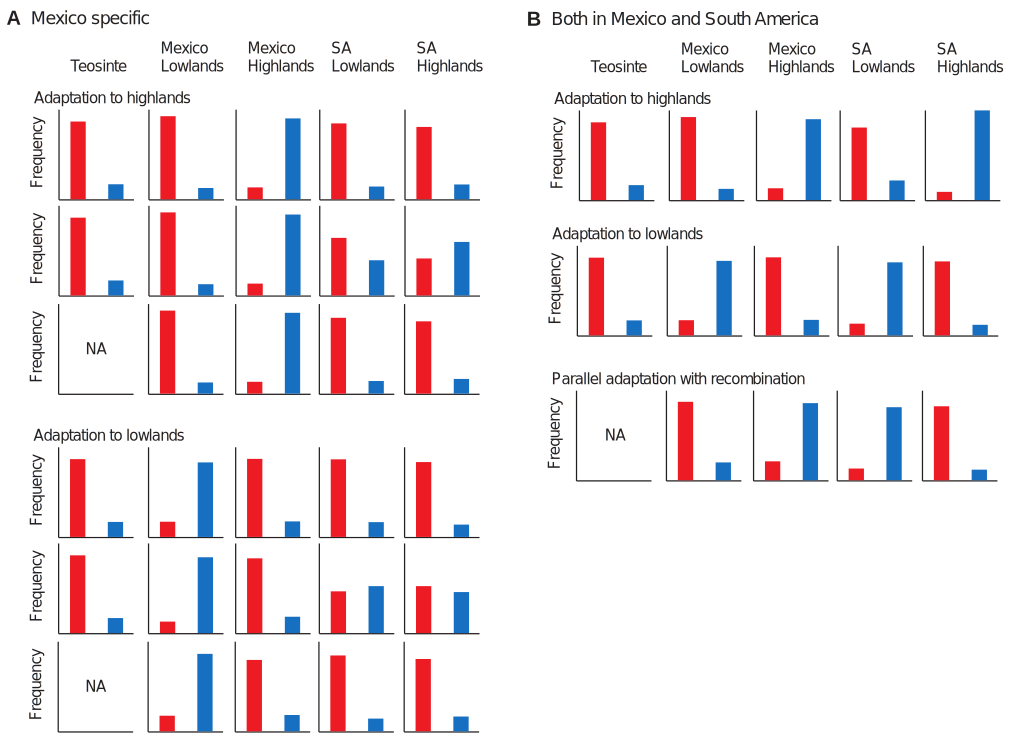
\includegraphics[width=0.49\textwidth]{fig/Fig7}
   \renewcommand{\baselinestretch}{0.9}
   \vspace{-3mm}
   \caption{Illustration for the typical patterns of allele frequency changes in teosinte and maize populations.  Red and blue bars represent the frequencies of putative ancestral and derived alleles, respectively.  (A) The pattern of allele frequencies in the SNPs with Mexico-specific significant $F_{ST}$ \emph{P}-values.  (B) The pattern of allele frequencies in the SNPs with significant $F_{ST}$ \emph{P}-values both in Mexico and South America.}
\vspace{-6mm}
    \label{tes2}
  \end{center}
\end{figure}
%%%%%%%%%%%%%%%%%%%%%%%%%%%%%%%%%%%%%%%%%% FIGURE









%We obtained teosinte (both  and \emph{mexicana}) SNPs in 46 of 56 SNPs from .  39 SNPs exhibited polymorphisms in teosinte, indicating selective sweep from standing genetic variation.  The other seven SNPs showed monomorphic in teosinte.  Only in two of seven SNPs, the frequencies of derived alleles were increased in highland populations. 


%%%%%%%%%%%%%%%%%%%%%%%%%%%%%%%%%%%%%%%%%%%%%%%%%%%%%%%%%%%%
\renewcommand{\arraystretch}{1.1}
\begin{table}[tb]

\begin{center}
 \caption[]{Introgression from \emph{mexicana}\hspace*{0.3cm}}
  \textbf{}\\[-2mm]
{\fontsize{7}{11}\sf
    \begin{tabular}{lcccccccl} 
    \hline
       & & \\[-3mm]
Mexico     & \multicolumn{3}{c}{Number of SNPs}  \\
                                  & Significant & NS & Proportion  \\
Introgressed regions & 149   &   1,918     & 0.072\\ 
Others                        & 872   &  73,578    & 0.011\\
      \hline
    & & \\[-3mm]
South America     & \multicolumn{3}{c}{Number of SNPs} \\
                                  & Significant & NS & Proportion  \\
Introgressed regions & 44   &   1703     & 0.025\\ 
Others      &703   &  60342    & 0.012\\[1mm]
    \hline
  %\multicolumn{4}{l}{$^{a}$ \textcolor{red}{Maybe we should use the number of genetic unit.}}\\
  % \multicolumn{4}{l}{$^{a}$ \textcolor{red}{Sum of the number of SNPs != 91,779 because I excluded SNPs exhibiting}}\\[-0.5mm]
  % \multicolumn{4}{l}{ \textcolor{red}{     monomorphic in Mexico or in South America.}}\\
    \end{tabular}
    \label{mex}  % caption is needed to make this work
}
\end{center}
\end{table}
\renewcommand{\arraystretch}{1}
%%%%%%%%%%%%%%%%%%%%%%%%%%%%%%%%%%%%%%%%%%%%%%%%%%%%%%%%%%%%


%%%%%%%%%%%%%%%%%%%%%%%%%%%%%%%%%%%%%%%%%%%%%%%%%%%%%%%%%%%%
\renewcommand{\arraystretch}{1.1}
\begin{table}[tb]

\begin{center}
 \caption[]{Tanja's $F_{CT}$ between \emph{parviglumis} and \emph{mexicana}\hspace*{0.3cm}}
  \textbf{}\\[-2mm]
{\fontsize{7}{11}\sf
    \begin{tabular}{lcccccccl} 
    \hline
       & & \\[-3mm]
Mexico     & \multicolumn{3}{c}{Number of SNPs}  \\
                                  & Significant & NS & Proportion  \\
Significant $F_{CT}$ & 31   &   331     & 0.086\\ 
NS                        & 373   &  18,419    & 0.020\\
      \hline
    & & \\[-3mm]
South America     & \multicolumn{3}{c}{Number of SNPs} \\
                                  & Significant & NS & Proportion  \\
Significant $F_{CT}$ & 12   &   325     & 0.036\\ 
NS                                & 250   &  17,401    & 0.014\\[1mm]
    \hline
  %\multicolumn{4}{l}{$^{a}$ \textcolor{red}{Maybe we should use the number of genetic unit.}}\\
  % \multicolumn{4}{l}{$^{a}$ \textcolor{red}{Sum of the number of SNPs != 91,779 because I excluded SNPs exhibiting}}\\[-0.5mm]
  % \multicolumn{4}{l}{ \textcolor{red}{     monomorphic in Mexico or in South America.}}\\
    \end{tabular}
    \label{tanja}  % caption is needed to make this work
}
\end{center}
\end{table}
\renewcommand{\arraystretch}{1}
%%%%%%%%%%%%%%%%%%%%%%%%%%%%%%%%%%%%%%%%%%%%%%%%%%%%%%%%%%%%

\subsection*{Comparison to theory}
\plr{need discussion of choices of selection coefficients?}

% # \mutrate computation:
% A <- 500; rho <- 5000; sb <- 10^(-(1:4)); xisq <- 50
% sapply( 10^c(-5,-8), function (mu) mu * (2 * rho * A * sb)/xisq )

Computing the rate $\mutrate$ at which newly adapted alleles arise in the population,
with at total population of $A \rho = 2.5 \times 10^6$ and an offspring variance of $\xi^2 = 50$,
we get that even if there is strong selection for the allele at high elevation ($s_b=0.1$),
then a single-base mutation with mutation rate $\mu=10^{-8}$ would still take at least 10,000 generations to appear and fix.
On the other hand, a kilobase-sized target with mutation rate $\mu=10^{-5}$
with this selection coefficient would fix in only 10 generations,
while more weakly selected alleles with $s_b$ of $10^{-2}$ or $10^{-3}$ would take hundreds or thousands of generations, respectively.
(note: at these values $\Tmut = 1/\mutrate = \mu s_b \times 10^5$.)

% # Tmig computation:
% A <- 500; rho <- 5000; sm <- 10^(-(1:4)); xisq <- 50; sigma <- 2
% 1/(sqrt(2*sm)/sigma)
% sapply( 1000*(1:4), function (R) 1 / ( A * rho * ( sqrt(2*sm) / xisq ) * exp(- sqrt(2*sm)*R/sigma ) ) )
% Ne <- (561/10^5)*A*rho 
% Ne  # = 14025
% sapply( 1000*(1:4), function (R) 1 / ( Ne * exp(- sqrt(2*sm)*R/sigma ) ) )

From the demographic model above
we have estimated that $\sigma \approx 2$ kilometers per generation,
so with $10^{-1} \ge s_m \ge 10^{-4}$ the distance $\sigma/\sqrt{2s_m}$ over which \eqref{eqn:migrate} decays 
is still short: between 4 and 150 kilometers.
\plr{put bounds on $\sigma$}
The area of the Andean highlands is about 500 km$^2$ \plr{is this right???}
which we estimate would be planted from around $N=14,000$ plants each year \plr{add more details here or above}.
Since the Mexican and Andean highlands are around 4,000 km apart,
at $s_m=10^{-3}$ the time needed for this to occur is $\Tmig \approx 5 \times 10^{34}$ generations.
In other words, from these calculations it is almost impossible that an allele that is deleterious at low elevation with $s_m=10^{-3}$ 
would ever transit from the Mexican to the Andean highlands.
If the selection against the allele is even weaker ($s_m=10^{-4}$) it is still expected to take $\Tmig = 1.8 \times 10^8$ generations.
However, shorter distances could be transited by very weakly deleterious alleles --
if $R$ is 1,000 km (or if $\sigma$ is four times larger)
then with $s_m=10^{-4}$ the time $\Tmig$ is about 1.6 generations --
so, adaptation by migration is certain.
However, with even $s_m=10^{-3}$ it is still $2.3 \times 10^6$ generations.

\plr{Here's my conclusions from these calculations.  But, maybe I'm missing something; I want to check more; tell me if anything seems awry.}
It seems unlikely that any alleles that are adaptive in the highlands and deleterious at all in the lowlands
would have transited central America by undirected (diffusive) sharing of seed.
The conclusions could change if we drastically underestimate the rate of very long distance sharing of seed,
e.g.\ if sharing across hundreds of kilometers was common at some point.

Both calculations are very pessimistic about the chance of shared single-base changes through either migration or independent mutation.
However, independent mutations could be expected in kilobase-size targets,
suggesting there might be signal for genes that share adaptive changes.

\plr{mesh this with data analysis\dots}
